%=============================================================================
\chapter{Path Planning Algorithms for Swarm Robots}\label{chap:algorithms}
%=============================================================================

This chapter reviews bio-inspired optimization methods that have been adapted for
decentralized, multi-robot path planning, emphasizing their natural inspirations,
their operational rules, and their adaptations to robot collectives for robust
and scalable navigation in dynamic environments.

Swarm intelligence approaches are popular in multi-robot settings because simple
local rules and indirect communication lead to emergent macroscopic behaviors
that remain robust to failures and scale to large populations without
centralized control \cite{nguyen2024swarm}.

%-----------------------------------------------------------------------------
\section{Bio-Inspired Algorithms}\label{sec:bio-inspired}

By mimicking foraging, flocking, and colony organization, bio-inspired algorithms
navigate complex spaces without a global model of the environment, thereby
achieving fast convergence and the ability to escape local minima for NP-hard
combinatorial objectives in multi-robot teams \cite{lin2022review}.

These methods rely on decentralized decisions by the agents, local perception,
and direct interaction or stigmergic signals, which together improve robustness,
scalability, and real-time responsiveness under the uncertainties common in
multi-robot deployments \cite{nguyen2024swarm}. Unlike planners that depend on an
explicit model of the environment, they let each robot act like an individual in
a natural collective, which favors decentralized decisions \cite{chen2025survey}.

\subsection{Ant Colony Optimization (ACO)}

ACO is a classical swarm intelligence method in which artificial ants deposit and
follow pheromone while constructing paths, steering the search toward promising
routes in large combinatorial spaces and in the motion graphs of robots
\cite{panigrahi2011handbook}.

Its core idea is positive feedback through pheromone reinforcement, combined with
evaporation to balance exploitation and exploration, which makes ACO well suited
to high-dimensional routing and discrete motion planning problems in robotics.

\subsubsection{Inspiration from Ant Foraging Behavior}

\begin{itemize}
  \item \lead{Pheromone mechanism} Real ants stochastically prefer paths with
        higher pheromone concentrations, so shorter paths accumulate pheromone
        faster and are chosen more often; the algorithm reproduces these dynamics
        of pheromone deposition and evaporation \cite{panigrahi2011handbook}.
  \item \lead{Stigmergic foundation} Trail laying and trail following constitute
        stigmergy---indirect coordination through modification of the
        environment---which in robotics can be implemented with virtual markers
        or distributed maps for decentralized navigation \cite{yi2019multi}.
\end{itemize}

\begin{figure}[htbp]
  \centering
  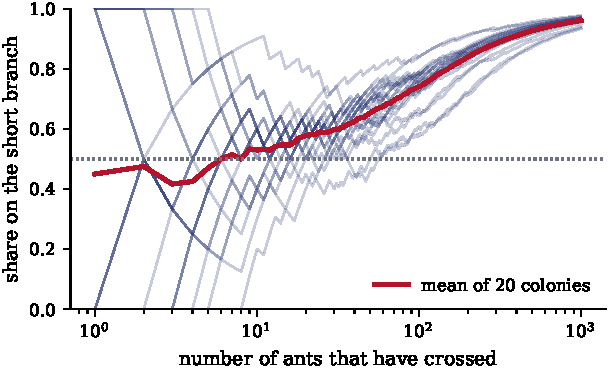
\includegraphics[width=0.72\linewidth]{aco-path-selection}
  \caption{A simulated double-bridge experiment: share of ants on the short
           branch for 20 colonies (thin lines) and their mean (thick line).
           Choices follow \cref{eq:trail-choice} with $k=20$, $\alpha=2$, and the
           long branch is twice as long, so it receives half the pheromone per
           crossing.}
  \label{fig:aco-path-selection}
\end{figure}

\Cref{fig:aco-path-selection} illustrates how ants select paths according to the
pheromone concentration. At first, there is no pheromone on either branch, so the
ants choose at random and the share on the short branch fluctuates around one
half. Because a round trip over the short branch is quicker, it is reinforced
more strongly per unit time (modelled here by a larger deposit), and the
pheromone difference grows. This positive feedback makes later ants prefer the
short branch, and after about a thousand crossings every simulated colony sends
more than 90\% of its traffic over it. These dynamics, which reproduce the
classical double-bridge experiments with real ants \cite{bonabeau1999swarm},
form the basis of ant colony optimization.

\subsubsection{Variants and Applications (AS-TSP, ACS-TSP)}

\begin{itemize}
  \item \lead{Ant System (AS-TSP)} The first ACO algorithm, proposed for the
        traveling salesman problem (TSP), which introduced the pheromone-guided
        constructive building of solutions but was later surpassed by improved
        variants \cite{dorigo1996ant}.
  \item \lead{Ant Colony System (ACS-TSP)} ACS strengthens AS with local pheromone
        updates, usually integrates local search such as 2-opt and 3-opt, and
        achieves leading performance, especially on the asymmetric TSP
        \cite{dorigo1997ant,bonabeau1999swarm}.
  \item \lead{Other applications} ACO variants have addressed quadratic
        assignment, sequential ordering, vehicle routing, and graph coloring
        problems. In robotics, ACO has been used to optimize the parameters of
        the membership functions of fuzzy controllers and, combined with fuzzy
        cost functions, for the navigation and path planning of mobile robots
        \cite{panigrahi2011handbook}. Together with PSO, ACO was one of the two
        mainstream paradigms of early swarm-intelligence research
        \cite{seebacher2025collective}.
\end{itemize}

\subsubsection{Pheromone Update Rules and Heuristics}

In standard ACO on graphs, a probabilistic transition rule weights the pheromone
intensity $\tau$ and the heuristic desirability $\eta$; pheromone evaporation and
a deposition proportional to the quality of the tour are then applied:
\begin{align}
  p_{ij}^{k}(t) &=
    \begin{cases}
      \dfrac{\tau_{ij}(t)^{\alpha}\,\eta_{ij}^{\beta}}
            {\sum_{u \in \mathcal{N}_i^{k}} \tau_{iu}(t)^{\alpha}\,\eta_{iu}^{\beta}},
        & j \in \mathcal{N}_i^{k}, \\[2ex]
      0, & \text{otherwise},
    \end{cases}
    \label{eq:aco-transition} \\[1ex]
  \eta_{ij} &= \frac{1}{d_{ij}},
    \label{eq:aco-heuristic} \\[1ex]
  \tau_{ij}(t+1) &= (1-\rho)\,\tau_{ij}(t) + \sum_{k=1}^{m} \Delta\tau_{ij}^{k},
    \label{eq:aco-update} \\[1ex]
  \Delta\tau_{ij}^{k} &=
    \begin{cases}
      \dfrac{Q}{L_k}, & \text{if } (i,j) \text{ is in the tour of ant } k, \\[1.5ex]
      0, & \text{otherwise}.
    \end{cases}
    \label{eq:aco-deposit}
\end{align}

In ACS, a local update that decreases the pheromone after each move lowers the
pheromone on recently used edges, which encourages exploration and prevents
premature stagnation \cite{panigrahi2011handbook}.

\subsubsection{Theoretical Aspects and Runtime Analysis}

\begin{itemize}
  \item \lead{Construction-graph model} ACO can be modeled as the construction of
        solutions on a graph with restricted transition neighborhoods and
        stochastic selection, which allows probabilistic runtime bounds to be
        derived, for example through fitness-level arguments
        \cite{gutjahr2007mathematical}.
  \item \lead{Convergence} Formal results show that the pheromones are bounded
        and that, with sufficient iterations and suitable parameter ranges, the
        probability of sampling optimal tours is positive; probabilistic
        convergence is thereby established for the basic ACO models
        \cite{gutjahr2007mathematical}.
  \item \lead{Controller tuning} Grid-based ACO has been used to tune the
        parameters of nonlinear PID (NLPID) controllers, and its convergence has
        been demonstrated in simulation loops for mechatronic systems, which
        illustrates the synergy between control and optimization
        \cite{panigrahi2011handbook}. The corresponding block diagram is shown in
        \cref{fig:aco-nlpid}.
\end{itemize}

\begin{figure}[htbp]
  \centering
  \tikzfigure[0.88\linewidth]{aco-nlpid}
  \caption{Using ACO to tune the parameters of an NLPID controller (redrawn after
           \cite{panigrahi2011handbook}).}
  \label{fig:aco-nlpid}
\end{figure}

\subsection{Particle Swarm Optimization (PSO)}

PSO models a swarm of particles that update their velocities and positions by
combining inertial motion, their personal best experience, and the social best,
yielding a simple yet powerful optimizer with strong empirical convergence and
low computational overhead \cite{nguyen2024swarm}.

Compared with many heuristics, PSO requires few parameters, is inherently
parallelizable, and is effective for continuous trajectory parameterization,
controller tuning, formation shaping, and multi-robot task allocation \cite{chen2019path}.

\subsubsection{Inspiration from Bird Flocking and Fish Schooling}

PSO was proposed by Kennedy and Eberhart in 1995 as a model of the social
behavior of bird flocks and fish schools \cite{kennedy1995particle}. Each particle
is a candidate solution in the search space, and its motion combines its current
velocity, the best position it has found itself (the personal best $p_i$), and
the best position found by the swarm or its neighborhood (the global best $g$).
This cognitive--social mechanism reflects alignment and cohesion in flocks and
schools, while inertia supports exploration
\cite{nguyen2024swarm,poli2007particle}:
\begin{equation}
  v_i^{t+1} = w\,v_i^{t} + c_1 r_1\left(p_i - x_i^{t}\right)
              + c_2 r_2\left(g - x_i^{t}\right), \qquad
  x_i^{t+1} = x_i^{t} + v_i^{t+1}, \qquad
  r_1, r_2 \sim U(0,1).
  \label{eq:pso}
\end{equation}

\subsubsection{Variants and Improvements (IPSO-DAI, NisB PSO)}

\begin{itemize}
  \item \lead{Parameter scheduling} Linearly decreasing the inertia weight $w$
        improves global exploration early in the search and local exploitation
        later on, reducing the risk of premature convergence in complex
        landscapes \cite{chen2019path}.
  \item \lead{PSO with integral control (IPSO-DAI)} Integral-controlled PSO
        (ICPSO) adds two integral controllers to the update to keep the
        population diverse; IPSO-DAI extends it with dispersed accelerator
        information, so that a predicted velocity index decides whether a particle
        moves in a divergent or a convergent manner. On high-dimensional
        multimodal benchmarks with many local optima, it outperformed standard
        PSO and ICPSO \cite{panigrahi2011handbook}.
  \item \lead{Topology} Ring topologies (lbest PSO) restrict the social
        neighborhood, and niching splits the swarm into sub-swarms (e.g., kPSO
        and NichePSO) that maintain multiple optima for multimodal path planning
        and multi-objective missions \cite{panigrahi2011handbook}; the robotic
        Darwinian PSO (RDPSO) uses the same idea of smaller sub-swarms to escape
        local optima with real robots \cite{dias2021swarm}.
  \item \lead{Hybrids} Combining PSO with B-spline smoothing, gravitational search,
        or symbiotic search improves compliance with kinematic/dynamic
        constraints and enhances the smoothness of solutions for flight and
        driving paths.
  \item \lead{Oscillating and collision-free PSO} Adding second-order/oscillatory
        terms together with collision-free constraints keeps the particles inside
        the feasible region in constrained navigation domains.
\end{itemize}

\subsubsection{Multi-Objective PSO (MOPSO)}

MOPSO generalizes single-objective PSO by replacing the single global best $g$
with archives of non-dominated solutions and with crowding or clustering
criteria that maintain a diverse Pareto front; it also redefines how the guides
for $p_i$ and for the group are selected, since with conflicting objectives there
is no single best position \cite{panigrahi2011handbook}. Representative variants
include:
\begin{itemize}
  \item \lead{Adaptive MOPSO (AMOPSO)} The inertia and acceleration coefficients
        are adapted over the iterations.
  \item \lead{Constrained adaptive MOPSO (CAMOPSO)} A penalty-based mechanism lets
        marginally infeasible solutions return to the feasible region, which
        helps when the feasible space is disconnected.
  \item \lead{Non-dominated sorting PSO (NSPSO)} Non-dominated sorting is used to
        rank the swarm and manage the front.
  \item \lead{Clustering} Clustering bounds the size of the archive and keeps the
        stored Pareto set well distributed.
\end{itemize}
A MOPSO generates a whole set of non-dominated solutions in one run, after which
fuzzy decision-making can pick the best compromise \cite{panigrahi2011handbook}.

\subsubsection{Application to UAV Swarm Path Planning}

\begin{itemize}
  \item \lead{Optimal paths} PSO plans short and safe paths for multiple vehicles
        while respecting obstacle and mission-time constraints; PSO formulations
        for simultaneous arrival and for minimizing mission time are common in
        multi-UAV scenarios \cite{he2021novel}. An example is shown in
        \cref{fig:pso-path}.
  \item \lead{Distributed control and reconnaissance} PSO updates have been used
        directly as the position commands of real quadcopters in swarm search
        \cite{lee2018realtime}; cooperative PSO generates safe, flyable paths for
        multi-UAV rendezvous that respect kinematic limits and are often smoothed
        with B-splines for curvature continuity \cite{lin2022review}.
  \item \lead{Controller and parameter tuning} Two-layer PSO frameworks tune the
        parameters of an inner target-tracking loop, while an outer loop
        optimizes the inner gains, enabling rapid gain synthesis across many
        geometric paths.
  \item \lead{Benchmarking} PSO is a standard baseline for comparison with newer
        bio-inspired methods (such as pigeon-inspired optimization) in aerial
        planning \cite{tan2016handbook,lin2022review}.
\end{itemize}

\begin{figure}[htbp]
  \centering
  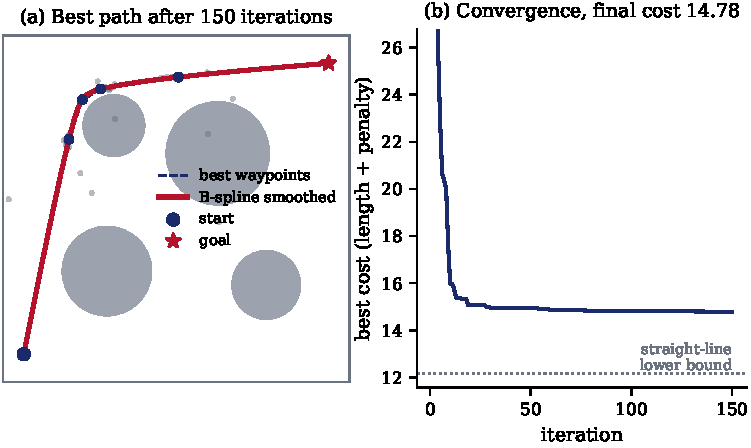
\includegraphics[width=\linewidth]{pso-path-planning}
  \caption{PSO path planning: each particle encodes four waypoints between the
           start and the goal, and the cost is the path length plus a penalty for
           entering an inflated obstacle. (a) The best waypoints after 150
           iterations, smoothed with a cubic B-spline; the grey dots are the final
           positions of the swarm. (b) Convergence of the best cost.}
  \label{fig:pso-path}
\end{figure}

\subsection{Bee-Inspired Algorithms}

Bee-inspired approaches mimic the division of labor and the recruitment of
foragers through waggle-dance-like communication in order to balance exploration
(scouts) and exploitation (employed and onlooker bees), producing robust global
search dynamics with few hyperparameters \cite{liang2015efficient}.

Honey-bee-based frameworks also include honey bee mating optimization (HBMO), the
Bees Algorithm (BA), and bee-colony-inspired methods tailored to discrete
constraints (e.g., time windows) in logistics \cite{liang2015efficient}.

\subsubsection{Honey Bees and the Artificial Bee Colony (ABC)}

ABC \cite{karaboga2005idea} divides the agents into employed bees (attached to food
sources, i.e., the current solutions), onlookers (which select sources
probabilistically according to their fitness), and scouts (which perform random
exploration or re-initialization after an abandonment limit is reached); with the
colony size and the number of cycles as its main control parameters, it delivers
robust performance \cite{panigrahi2011handbook}.

Its advantages include simplicity, robustness, and a small set of parameters,
although the search can slow down near the optimum and diversity can decrease.
Variants such as BCiA (for the vehicle routing problem with time windows,
VRP-TW) and BA (for training neural networks) adjust the balance between
exploration and exploitation and the problem encoding for discrete settings
\cite{panigrahi2011handbook}.

\subsubsection{Hierarchical and Multi-Island ABC Models}

Parallel and distributed ABC variants, by offloading evaluations, sharing elite
solutions, and co-evolving subpopulations, improve the scalability of
high-dimensional path planning, reducing the wall-clock time while preserving
diversity \cite{panigrahi2011handbook}.
\begin{itemize}
  \item \lead{Master--worker ABC} Central coordination parallelizes costly
        evaluations and local searches on worker nodes to accelerate
        time-critical planning \cite{panigrahi2011handbook}.
  \item \lead{Multi-hive (multi-island) ABC} Independent hives periodically
        migrate elite solutions and, through co-evolution, raise the quality of
        the solutions while containing the growth of computation
        \cite{panigrahi2011handbook}.
  \item \lead{Hierarchical--hybrid ABC (HH-ABC)} Islands exchange elites at the
        upper level, and each island internally runs a master--worker ABC,
        combining diversification with parallel speedup at large scale
        \cite{panigrahi2011handbook}.
\end{itemize}
In comparisons with an enhanced sequential ABC that also uses local search, the
parallel and multi-population models consistently reached good solutions with
less computation on problems with many variables \cite{panigrahi2011handbook}.

\subsection{Other Swarm Intelligence Algorithms}

Many other natural metaphors have produced metaheuristics that are used for
high-dimensional planning and optimization in swarm robotics
\cite{shahzad2023review,nguyen2024swarm}.

\subsubsection{Firefly, Flower Pollination, and Artificial Flora Algorithms}

In the firefly algorithm (FA), the brightness of a firefly encodes the quality of
its solution, and a dimmer firefly moves toward a brighter one, so the
population gathers around the best individual \cite{yang2009firefly}. A common
form of the update is
\begin{equation}
  x_i \leftarrow x_i + \beta_0\, e^{-\gamma r_{ij}^{2}} \left(x_j - x_i\right)
        + \alpha\, \epsilon_i,
  \label{eq:firefly}
\end{equation}
where $r_{ij}$ is the distance between fireflies $i$ and $j$, $\beta_0$ is the
attractiveness at zero distance, $\gamma$ is the light absorption coefficient,
and the random term $\alpha \epsilon_i$ keeps the search from stagnating. The
flower pollination algorithm (FPA) imitates the global and local pollination of
flowering plants \cite{yang2012flower}, and the related artificial flora (AF)
algorithm imitates how plants spread seeds over an area to find the best place to
grow, generating ``offspring plants'' around an ``original plant'' with
propagation functions; in its authors' comparisons, AF was more stable and
accurate than PSO and ABC \cite{cheng2018artificial}.

\subsubsection{Fireworks and Dragonfly Algorithms}

The fireworks algorithm (FWA), introduced by Tan, models the explosion of
fireworks: good solutions act as explosion sites around which ``sparks''
(new candidate solutions) are generated to refine the search \cite{tan2010fireworks}.
The guided fireworks algorithm reappears in \cref{sec:learning} as the optimizer
of a learned search policy. The dragonfly algorithm imitates the static and
dynamic swarming of dragonflies \cite{mirjalili2016dragonfly}, and its strategy
parameters have been tuned to make multi-target search by robot swarms more
efficient \cite{bhowmick2024bio}.

\subsubsection{Glowworm Swarm Optimization (GSO)}

GSO is designed for multimodal problems in which several optima, or several
sources, must be found at once. Each glowworm carries a luminescence quantity,
\emph{luciferin}, which grows with the fitness $J$ at its position and decays
over time,
\begin{equation}
  \ell_i(t+1) = (1-\rho)\,\ell_i(t) + \gamma\, J\bigl(x_i(t+1)\bigr),
  \label{eq:gso}
\end{equation}
and each agent moves toward a brighter neighbor within an adaptive decision
range. Because distant individuals have no influence, the swarm splits
automatically into sub-swarms around the different optima. GSO has been used
for localizing multiple odor sources and tracking mobile signal sources with
groups of robots \cite{krishnanand2009glowworm,panigrahi2011handbook}.

\subsubsection{Distributed Hybrid Fish Swarm Optimization (DHFSOA)}

DHFSOA is an example of the trend toward specialized, hybrid swarm algorithms.
Based on the collective search of fish schools, it was proposed for event-driven
sensor deployment in underwater acoustic sensor networks, where conventional
redeployment algorithms become complicated, and it finds good deployments faster
than traditional methods \cite{wang2018event}.

%-----------------------------------------------------------------------------
\section{Graph-Based and Sampling-Based Methods}\label{sec:graph-sampling}

Graph- and sampling-based planners convert continuous motion planning into a
tractable discrete search by building graphs or trees in the free space; this
approach is particularly effective in high-dimensional or geometrically complex
environments, where cell grids or potential fields struggle \cite{abujabal2024path}.

These methods offer probabilistic completeness or strong practical performance
while remaining compatible with the decentralized execution that is common in
swarms \cite{lin2022review}.

\subsection{Probabilistic Roadmap (PRM)}

PRM is a classical multi-query sampling-based planner that builds a roadmap of
sampled collision-free configurations and connects them with local planners; it
then links the start and goal points to the roadmap and finds a path through
graph search \cite{kavraki1996probabilistic}. Its multi-query nature and
relatively low query cost have made PRM a common backbone that is combined with
metaheuristics or behavioral rules in multi-robot systems and swarms
\cite{neto2017multi,lin2022review}. Complete planners, which find a path or prove
that none exists, need time that grows exponentially with the number of degrees
of freedom, which is why randomized methods such as PRM are preferred in high
dimensions \cite{kavraki1996probabilistic}.

\subsubsection{Roadmap Construction in High-Dimensional Spaces}

PRM tames the exponential growth of the configuration space with increasing
degrees of freedom by random sampling, approximating the connectivity of $\Cfree$
without an exhaustive search. The pipeline has two phases: a preprocessing phase,
which builds the roadmap by sampling collision-free milestones and connecting
nearby neighbors with a simple local planner, and a query phase, which connects
the start and goal to the roadmap and runs a graph search for a feasible path
\cite{neto2017multi}.

The roadmap approximates a graph over $\Cfree$ whose vertices are the milestones
and whose edges are feasible local connections; its completeness is
probabilistic and improves with the number of samples and the connection radius
\cite{neto2017multi}.
\begin{itemize}
  \item \lead{Managing complexity} Performance depends on the number and
        placement of the milestones; informed samplers such as Medial-Axis PRM
        (MAPRM) bias the samples toward the medial axis to increase safety
        margins, yielding higher-quality roadmaps with fewer samples
        \cite{sahin2005swarm}.
\end{itemize}

\begin{figure}[htbp]
  \centering
  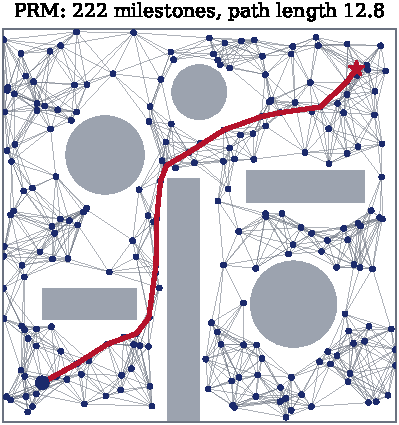
\includegraphics[width=0.55\linewidth]{prm-example}
  \caption{PRM in a cluttered workspace: collision-free milestones are connected to
           their ten nearest neighbours, and Dijkstra's algorithm finds the path on
           the roadmap.}
  \label{fig:prm}
\end{figure}

\subsubsection{Integration with Flocking and Shepherding}

Roadmaps inject a global navigation structure into swarms that interact mainly
locally, enabling coordinated homing, exploration and coverage, passage through
narrow corridors, and shepherding strategies.\footnote{Shepherding: an external
agent selects a path on the roadmap and, by issuing commands, guides the swarm
along it, so that global guidance is blended with the local cohesion of the
flock \cite{sahin2005swarm}.} Flocks can traverse the edges of the roadmap while node-level
rules for separation, alignment, and cohesion preserve the formation and spacing,
especially in narrow regions or bottlenecks \cite{sahin2005swarm}. Roadmaps have
supported several group behaviors:
\begin{itemize}
  \item \lead{Homing and goal searching} The roadmap gives the flock the
        structure it needs to reach a known goal or to search for an unknown one.
  \item \lead{Exploration and coverage} The edges gain weight as robots traverse
        them, and at each junction the flock chooses probabilistically in favor of
        lower-weight edges, so less-visited corridors get priority.
  \item \lead{Narrow passages} Roadmap nodes can carry rules that the flock
        members apply when they reach them, which coordinates the flock's
        configuration in narrow or complex areas.
  \item \lead{Shepherding} An external agent extracts a path from the roadmap and
        steers the flock from behind along it.
\end{itemize}

\subsection{Rapidly-Exploring Random Trees (RRT)}

RRT samples the state space and greedily extends a tree from the nearest node
toward each sample, rapidly exploring unknown regions and quickly producing
feasible (though not necessarily optimal) paths
\cite{lavalle1998rapidly,abujabal2024path}.

RRT is probabilistically complete and accommodates kinodynamic constraints, which
makes it practical for robots with dynamics and control limitations.

\subsubsection{RRT and RRT-Connect for Single-Agent Queries}

RRT views motion planning as a tree search that expands toward uniform samples
and connects new states to their nearest neighbor using a local steering function
subject to the constraints \cite{lavalle1998rapidly}.

RRT-Connect grows two trees, one from the start and one from the goal, and
aggressively attempts to join them with its CONNECT heuristic, which reduces the
search time compared with a single tree \cite{kuffner2000rrt}. \RRTstar{} adds a
rewiring step that makes the solution asymptotically optimal, at a higher
computational cost \cite{karaman2011sampling}. The difference between RRT and
RRT-Connect can be seen in \cref{fig:rrt}.

\begin{figure}[htbp]
  \centering
  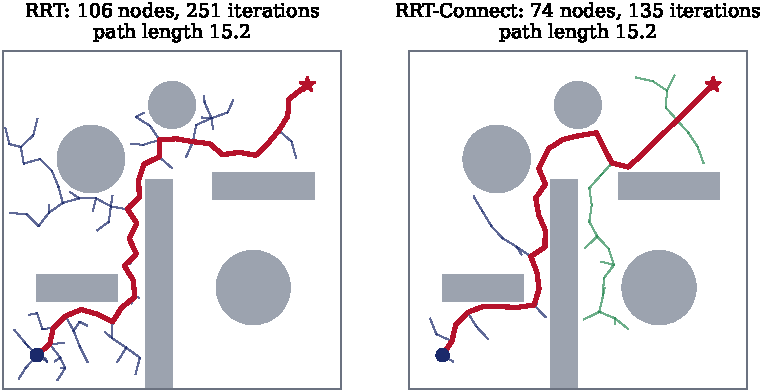
\includegraphics[width=0.95\linewidth]{rrt-vs-rrt-connect}
  \caption{RRT and RRT-Connect in the workspace of \cref{fig:prm}, with the same
           step size and random seed. RRT-Connect grows a tree from each end and
           joins them with its CONNECT step, so it needs fewer iterations.}
  \label{fig:rrt}
\end{figure}

\subsubsection{Adaptations for Swarm Robotics (e.g., Virtual Tubes)}

Distributed RRT enables decentralized collision avoidance: each agent plans while
accounting for the other agents and the static obstacles, using local
communication when needed \cite{lin2022review}.

In dynamic environments, \emph{grafting}---inserting new intermediate waypoints
into an existing RRT path when the obstacles change---avoids complete replanning
and enables real-time updates for multi-robot teams \cite{li2021rrt}.
\begin{itemize}
  \item \lead{Optimal virtual tube planning (OVTP) and Tube-\RRTstar} A
        hierarchical approach first generates homotopic paths (e.g., with
        \RRTstar) and then builds an ``optimal virtual tube'' that bounds safe,
        obstacle-free corridors for the synthesis of a central path and for
        distributed execution; Tube-\RRTstar{} trades off path length against the
        cross-sectional area of the corridor in order to contain the swarm
        \cite{mao2023optimal,mao2024tube}.
\end{itemize}
The computational complexity of tube planning is
\begin{equation}
  O\bigl(n(\log n + 1) + l\bigr),
  \label{eq:tube-complexity}
\end{equation}
for $l$ homotopic paths on $n$ samples, compared with
\begin{equation}
  O\bigl(n\,l\,(\log n + 1)\bigr)
  \label{eq:multipath-complexity}
\end{equation}
when \RRTstar{} is simply run $l$ times \cite{mao2024tube}.

\subsubsection{Sub-Optimal Algorithms for Higher Speed}

\begin{itemize}
  \item \lead{Multi-tree structures} Bidirectional RRT-Connect and three-tree
        approaches parallelize exploration from multiple fronts and improve the
        success rate in narrow passages \cite{abujabal2024path,yuan2020bilevel}.
  \item \lead{Biased sampling} Goal biasing accelerates convergence;
        obstacle-biased methods (e.g., Dangerzone RRT) steer the samples toward
        the boundaries of obstacles so that narrow corridors are traversed
        efficiently.
  \item \lead{Roadmap-guided sampling} GVD-guided RRT uses the generalized
        Voronoi diagram (GVD) as a heuristic backbone and greatly accelerates
        planning in maze-like scenes.
  \item \lead{Dynamic replanning} DRRT prunes and repairs only the invalidated
        parts of the path when changes occur; ERRT resumes growth when the path
        is blocked; and multipartite RRTs (MPRRT) combine fast pruning with
        restart behavior to maintain responsiveness \cite{chen2025survey}.
  \item \lead{Pseudo-random trees} The multi-agent rapidly-exploring pseudo-random
        tree replaces random sampling with a deterministic sequence, keeping
        probabilistic completeness while converging quickly
        \cite{neto2017multi}.
\end{itemize}

\subsection{The \texorpdfstring{\Astar}{A*} Algorithm and Grid-Based Methods}

Deterministic graph and grid planners are fundamental for structured maps:
\Astar{} yields optimal paths with the help of heuristics, and grids and cell
decompositions provide discrete models that are suited to proofs of correctness
and to integration with other planners. These methods are often used as
baselines or as components of hybrid multi-robot path planning systems
\cite{abujabal2024path,lin2022review}.

\subsubsection{\texorpdfstring{\Astar}{A*} for Optimal Paths in Static Environments}

\Astar{} evaluates nodes with $f(n) = g(n) + h(n)$, where $g(n)$ is the cost from
the start and $h(n)$ is an admissible heuristic estimate of the cost to the goal;
this guarantees completeness and optimality on graphs with nonnegative edge
weights \cite{hart1968formal}. An example of how this method works is shown in
\cref{fig:astar}; its weakness is that the search effort still grows quickly as
the search space expands \cite{abujabal2024path}.

With informed heuristics, \Astar{} is more efficient than Dijkstra's algorithm in
large spaces, and it is often combined with fuzzy neural networks to speed up
task completion and improve controllability and adaptability in multi-robot
systems \cite{tan2016handbook}.

\begin{figure}[htbp]
  \centering
  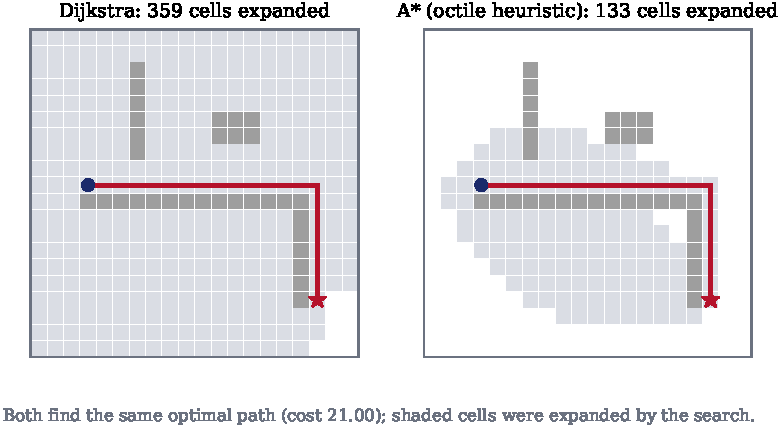
\includegraphics[width=0.9\linewidth]{astar-grid}
  \caption{Dijkstra's algorithm and \Astar{} on the same 8-connected grid. Both
           return the same optimal path, but the admissible octile heuristic lets
           \Astar{} expand far fewer cells.}
  \label{fig:astar}
\end{figure}

\subsubsection{Grid-Based Environment Representation}

Grid maps discretize space into cells, turning continuous motion into a graph
search for algorithms such as \Astar, \Dstar, or even ACO on grids, and they can
be updated online to handle dynamics \cite{abujabal2024path}. The resolution is a critical
trade-off between accuracy and computation or memory: a very fine grid is
expensive and a very coarse one is inaccurate, which is why multi-resolution or
hierarchical grids are attractive in practice \cite{lin2022review}.

\subsubsection{Cell Decomposition Techniques (e.g., Boustrophedon, Morse)}

Cell decomposition partitions $\Cfree$ into non-overlapping cells and builds an
adjacency graph whose nodes are the cells and whose edges are adjacency
relations; optimal paths are obtained by a graph search across the cells with
methods such as Dijkstra's algorithm or \Astar{} \cite{abujabal2024path}.

Boustrophedon decomposition supports exact coverage by sweeping and splitting the
space at points where its connectivity changes \cite{choset2000coverage}, whereas
Morse decompositions use the critical points of a Morse function to produce cells
that are easily covered with simple back-and-forth patterns once entered
\cite{acar2006sensor}.

\subsubsection{Generalized Voronoi Diagrams (GVD) for Narrow Regions}

The GVD partitions the free space into loci that are equidistant from the
obstacles: its edges are the points equidistant from two obstacles, and its meet
points are equidistant from three or more. By maximizing the safety margin, these
edges and junctions serve as a roadmap for safe passage through cluttered
environments and narrow passages \cite{acar2006sensor,breitenmoser2010voronoi}.

Planning can move along the GVD, reach its edges near the goal, and then exit
toward the goal. The GVD also guides sensor-based coverage, accelerates RRT in
maze-like environments, and supports path-priority strategies for multiple robots
in narrow passages \cite{breitenmoser2010voronoi}.

\begin{figure}[htbp]
  \centering
  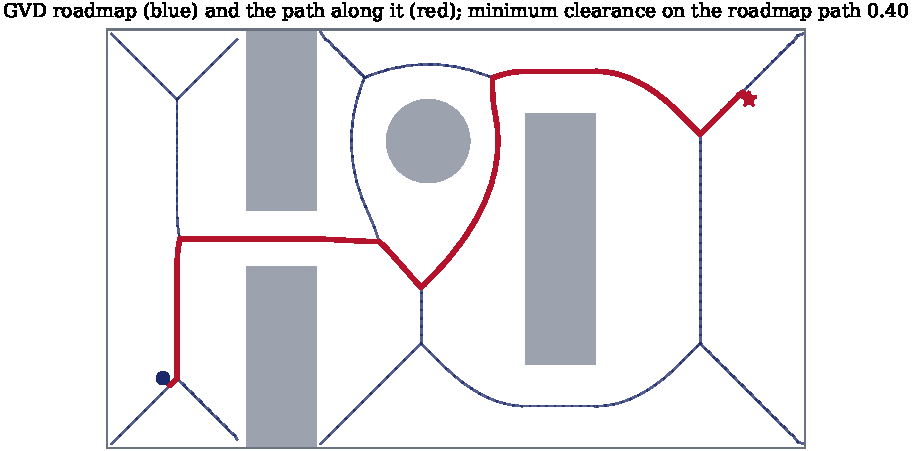
\includegraphics[width=0.85\linewidth]{voronoi-narrow-regions}
  \caption{An approximate generalized Voronoi diagram, built from the ordinary
           Voronoi diagram of points sampled on the obstacle boundaries. The path
           follows the roadmap through the narrow door and keeps the largest
           possible distance from the walls.}
  \label{fig:voronoi}
\end{figure}

%-----------------------------------------------------------------------------
\section{Potential Field Methods}\label{sec:potential-fields}

Potential field planners, and particularly the artificial potential field (APF),
turn path planning into gradient-following motion by defining deterministic,
rule-based potentials. Their simplicity, fast computation, and real-time
reactivity in dynamic scenes make them attractive for distributed swarms
\cite{nazarahari2019multi}.

In multi-robot systems, the APF is usually employed as a local planner or control
law that integrates smoothly with higher-level graph or sampling planners or with
metaheuristics, keeping the computational cost per agent low while preserving
decentralized execution \cite{wang2022coordination}.

\subsection{Artificial Potential Fields (APF)}

The APF, pioneered by Khatib in 1986, remains the standard for geometric
navigation based on force fields: the goal creates attraction in the
configuration space, the obstacles create repulsion, and the motion commands are
derived from the negative gradient of the potential \cite{khatib1986real}.

In multi-agent settings, the APF models inter-agent and agent--environment
interactions as attractive--repulsive potentials, and gradient-based controls
ensure formation, tracking, and collision avoidance with decentralized feedback
\cite{wang2018research}.

\subsubsection{Attractive and Repulsive Forces for Navigation}

The APF defines a total potential $U(X)$ as the sum of attractive and repulsive
components and computes the net control force as the negative gradient of this
potential, so that the robot descends toward the goal while keeping away from the
obstacles:
\begin{equation}
  U(X) = U_{\att}(X) + U_{\rep}(X), \qquad
  F(X) = -\nabla U(X) = F_{\att}(X) + F_{\rep}(X).
  \label{eq:apf}
\end{equation}
Here, $U_{\att}$ pulls the agent toward the goal, and $U_{\rep}$ increases sharply
near the obstacles to preserve safety, providing smooth closed-loop motion that
is suitable for real-time embedded control \cite{wang2022coordination}. A common
attractive potential is quadratic, $U_{\att}(X) = \tfrac{1}{2} k_{\att}
\|X - X_g\|^2$, and a typical repulsive potential is
\begin{equation}
  U_{\rep}(X) =
  \begin{cases}
    \dfrac{1}{2}\,k_{\rep}\left(\dfrac{1}{d(X)} - \dfrac{1}{d_0}\right)^{2},
      & d(X) \le d_0, \\[2.5ex]
    0, & d(X) > d_0.
  \end{cases}
  \label{eq:apf-repulsive}
\end{equation}
Consequently, $\|\nabla U_{\rep}\|$ grows without bound as $d(X) \to 0$, which
gives priority to collision avoidance near the boundaries \cite{zhao2020multi}.

\begin{figure}[htbp]
  \centering
  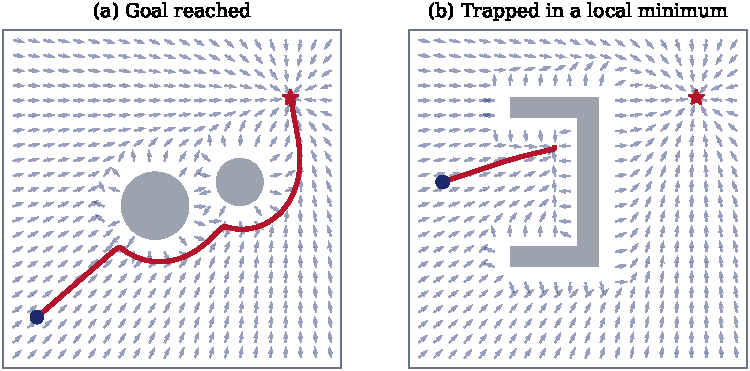
\includegraphics[width=\linewidth]{apf-forces}
  \caption{The force-field view of robot path planning: the arrows show the
           direction of $F = -\nabla U$. (a) The target attracts and the
           obstacles repel the robot, which reaches the goal. (b) A U-shaped
           obstacle creates a local minimum in which the same controller gets
           stuck.}
  \label{fig:apf}
\end{figure}

\subsubsection{Principles of Obstacle Avoidance and Goal Seeking}

\begin{itemize}
  \item \lead{Goal seeking} $U_{\att}(X)$ is shaped so that the magnitude of the
        attractive force is large far from the goal and zero at the goal; this
        ensures natural deceleration and stopping at the potential minimum and
        encodes precise capture of the goal in static scenes \cite{wang2022coordination}.
  \item \lead{Obstacle avoidance} $U_{\rep}(X)$ grows rapidly as the distance to
        the obstacles decreases and can vanish outside a radius of influence;
        this design enforces separation because the repulsive gradient dominates
        near the boundaries \cite{wang2018research}.
  \item \lead{Known limitations} The classical APF may suffer from local minima
        and is sensitive to parameter tuning, which can trap the robot away from
        the global minimum; hybridization or adaptive shaping is commonly used in
        practice to mitigate this problem \cite{zhao2020multi}.
\end{itemize}

\subsubsection{Improved Potential Field for Cooperative Target Hunting}

To overcome local minima and embed multi-robot cooperation, improved potential
fields (IPFs) add cooperation measures and problem-specific shaping, which enables
coordinated target hunting by multi-AUV teams in turbulent, dynamic surface-water
environments \cite{ge2018multi}. The cooperation is expressed through three
measures: a dispersion degree $H_D$ that spreads the agents apart, a homodromous
degree $H_H$ that keeps their headings consistent, and a district-difference
degree $H_{DD}$ that distributes the search; a term in the relative distance to
the target makes sure that the only global minimum is at the target, which
removes the local-minimum problem \cite{ge2018multi}.

A representative formulation of the total potential for AUV $R_i$ is the weighted
combination
\begin{equation}
  U_i = \omega_{\alpha}\,U_{\alpha} + \omega_{\gamma}\,U_{\gamma},
  \label{eq:ipf-total}
\end{equation}
where the attractive component $U_{\alpha}$ covers the exploration and
target-tracking phases, and the repulsive component $U_{\gamma}$ combines
cooperation degrees for dispersion, heading alignment (homodromy), and district
difference (spatial distribution) with the density weights $\omega_{\gamma D}$,
$\omega_{\gamma H}$, and $\omega_{\gamma DD}$ \cite{ge2018multi}.

The attractive component is defined piecewise as
\begin{equation}
  U_{\alpha}\left(X_{R_i}\right) =
  \begin{cases}
    \dfrac{1}{2}\,k_1\,\Phi\!\left(\dfrac{N_u}{N}, \dfrac{A}{\bar{A}}\right),
      & \text{exploration}, \\[2.5ex]
    \dfrac{1}{2}\,k_2 \left\| X_{R_i} - X_{T_l} \right\|^{2},
      & \text{moving to the target},
  \end{cases}
  \label{eq:ipf-attractive}
\end{equation}
where $\Phi$ increases with the proportions of undetected targets and unexplored
areas, and the target-tracking term uses a quadratic pull toward the assigned
target $T_l$ \cite{ge2018multi}.

The repulsive and cooperative component is defined as
\begin{equation}
  U_{\gamma} =
  \begin{cases}
    \omega_{\gamma D} H_D + \omega_{\gamma H} H_H + \omega_{\gamma DD} H_{DD},
      & \text{exploration}, \\[1.5ex]
    \dfrac{1}{2}\,\kappa \left(\dfrac{1}{d} - \dfrac{1}{d_1}\right)^{2}
      + \text{(cooperation terms)},
      & \text{near obstacles},
  \end{cases}
  \label{eq:ipf-repulsive}
\end{equation}
where $H_D$ encourages spacing, $H_H$ increases the coherence of headings, and
$H_{DD}$ promotes spatial distribution to prevent excessive concentration; the
obstacle term explicitly maintains the safety margin \cite{ge2018multi}.

Performance evidence from Monte Carlo experiments with six AUVs, two dynamic
targets, and obstacles in a $120 \times 120~\mathrm{m}^2$ area shows that the IPF
reduces the path length and the hunting time compared with the classical
potential field, indicating greater efficiency, robustness, and cooperation even
when agents fail. The IPF also maintained high success rates under random layouts
and dynamics, and it outperformed baseline PSO methods in obstacle-rich hunts
while preserving collision-free pursuit and distributed coordination \cite{ge2018multi}.

%-----------------------------------------------------------------------------
\section{Reinforcement Learning and Deep Learning Approaches}\label{sec:learning}

AI learning methods take path planning beyond fixed rules by allowing agents to
optimize their behavior through experience, which makes them robust to
uncertainty and environmental change in multi-robot systems. Reinforcement
learning (RL) and its extensions are widely used for decentralized
decision-making, real-time collision avoidance, and cooperative tasks in swarms
\cite{he2021integral}.

\subsection{Reinforcement Learning (RL)}

RL formulates sequential decision-making as the optimization of the expected
cumulative reward through repeated interaction with the environment, enabling
data-driven improvement without labeled datasets. This adaptability makes RL
effective in the dynamic, partially known, or adversarial environments that are
common in real-world multi-robot deployments.

\subsubsection{Learning Optimal Behaviors through Trial and Error}

Agents learn policies $\pi(a \mid s)$ that maximize the objective
\begin{equation}
  \max_{\pi}\; \mathbb{E}_{\pi}\!\left[\sum_{t=0}^{\infty} \gamma^{t} r_t\right],
  \qquad \gamma \in (0,1),
  \label{eq:rl-objective}
\end{equation}
while exploration strategies ensure sufficient coverage of the state--action space
during learning.

Policy optimization can be value-based, policy-gradient, or actor--critic, and it
is chosen according to the complexity of the task, the observability, and the
properties of the action space. The goal of policy optimization is to compute a
mapping $\pi^{*} : S \to A$ that maximizes the long-term return under the dynamics
of the environment while balancing exploration and exploitation.
\begin{itemize}
  \item \lead{Adaptability} RL adapts to environmental changes by continuously
        updating value functions or policy parameters, maintaining performance in
        situations where classical planners would need costly replanning.
  \item \lead{Learning without labels} RL does not require supervised learning
        with labels; agents learn from numerical rewards that encode the task
        objectives and safety constraints.
\end{itemize}

\subsubsection{Optimal Flight Paths for UAV Swarms}

Multi-agent RL (MARL) with centralized training and decentralized execution
(CTDE) supports cooperative navigation by training shared critics or common value
baselines, while decentralized policies run on the individual UAVs
\cite{azzam2023swarm,lowe2017multi}.

MARL policies compute efficient coverage and routing for various map sizes and
swarm sizes, improving mission time and battery consumption compared with
hand-crafted rules \cite{xue2021multi}.
\begin{itemize}
  \item \lead{Cooperative navigation} CTDE allows agents to learn coordination
        (e.g., collision-free formations and simultaneous arrival) while keeping
        run-time control decentralized. This scheme is shown in \cref{fig:ctde}.
  \item \lead{Coverage optimization} Learned policies maximize the reward for
        first-visited cells and minimize repeated traversal, achieving scalable
        area coverage \cite{xue2021multi}.
  \item \lead{Hybrids and speed} Neural-network function approximation
        accelerates Q-learning; a global neural network and heuristic Q-learning
        variants speed up convergence and reduce the hardware requirements for
        on-board deployment \cite{lin2022review}.
\end{itemize}

\begin{figure}[htbp]
  \centering
  \tikzfigure[0.85\linewidth]{ctde}
  \caption{The CTDE scheme: a centralized critic is trained on the observations
           and actions of all agents, while each agent executes its own
           decentralized actor.}
  \label{fig:ctde}
\end{figure}

\subsubsection{Rewards and Interaction with the Environment}

Reward design directly steers the learning process and must encode safety,
efficiency, and cooperation for swarms. In coverage tasks, first-time visits
usually receive larger rewards, collisions, oscillations, and deadlocks are
penalized, and shaping terms are added to speed up learning.
\begin{itemize}
  \item \lead{Incentive mechanism} Positive rewards for progress toward the goal
        and for coverage, and negative rewards for collisions or constraint
        violations, lead to a stable improvement of the policy.
  \item \lead{Credit assignment} Global team rewards can mask individual
        contributions (``lazy agents'') and make credit assignment difficult in
        swarms.
  \item \lead{Solutions} Local rewards, heterogeneous reward components, and
        difference rewards or agent-specific critics factor global objectives
        into per-agent feedback, improving the stability and fairness of
        learning.
\end{itemize}

\subsection{Deep Reinforcement Learning (DRL)}

DRL, by integrating deep neural networks with RL, handles the high-dimensional
observations, partial observability, and continuous control that are common in
robotics and swarms. DRL reduces the reliance on static maps by learning from raw
or learned features, and it supports real-time inference on embedded
accelerators \cite{zhang2025deep}.

\subsubsection{Path Planning in Complex and Dynamic Environments}

DRL scales to dynamic obstacles and narrow passages, where classical methods face
slow convergence or limited representational capacity \cite{zhang2025deep}.

Typical progressions include the deep Q-network (DQN), whose experience replay
improved data efficiency \cite{mnih2015human}, and Double DQN for greater
stability, followed by actor--critic methods for continuous actions, such as DDPG
and TD3, which adds double Q-learning to DDPG \cite{zhang2025deep,fujimoto2018addressing}.
\begin{itemize}
  \item \lead{High dimensionality} DRL learns collision avoidance and multi-agent
        coordination directly from sensor and state embeddings, without
        hand-crafted features or complete global maps \cite{huttenrauch2019deep}.
  \item \lead{Limits of value-based approaches} DQN and Double DQN struggle in
        continuous action spaces; policy-gradient methods (DDPG, TD3) mitigate
        this problem, but TD3 relies on injected noise and may under-explore in
        complex terrains \cite{zhang2025deep}.
\end{itemize}

\subsubsection{Soft Actor-Critic (SAC) Algorithms for Continuous Actions}

SAC promotes robust exploration in continuous control by maximizing a
maximum-entropy objective, jointly optimizing the expected return and the entropy
of the policy \cite{haarnoja2018soft,zhang2025deep}:
\begin{equation}
  J(\pi) = \mathbb{E}_{\pi}\!\left[\sum_{t=0}^{\infty} \gamma^{t}
           \Bigl(r_t + \alpha\, \mathcal{H}\bigl(\pi(\cdot \mid s_t)\bigr)\Bigr)\right],
  \qquad \alpha > 0.
  \label{eq:sac}
\end{equation}
\begin{itemize}
  \item \lead{Exploration and robustness} Entropy regularization reduces
        premature convergence to sub-optimal behaviors and improves performance
        under non-stationary conditions.
  \item \lead{Advanced variants (e.g., GAP\_SAC)} GAP\_SAC combines a dynamic
        heuristic reward inspired by heuristic search, which gives a smooth
        signal toward the goal, with prioritized experience replay and a gated
        attention mechanism that focuses the network on the important features
        of the environment. In dynamic and narrow scenarios it produced shorter
        paths and converged faster than SAC and TD3 \cite{zhang2025deep}.
  \item \lead{Prioritized replay} Transitions are prioritized according to their
        temporal-difference (TD) error, and the resulting replay bias is
        corrected through importance sampling \cite{schaul2016prioritized}:
        \begin{equation}
          P(i) \propto \left|\delta_i\right|^{\alpha}.
          \label{eq:per}
        \end{equation}
  \item \lead{State augmentation} Adding features such as the Euclidean distance
        to the goal (DG) and the amount of heading correction (MA) improves
        observability and planning performance for mobile robots \cite{zhang2025deep}.
\end{itemize}

\subsection{Imitation Learning (IL)}

Imitation learning (IL), or learning from demonstration, learns policies from
expert trajectories: instead of optimizing an unknown reward, it minimizes the
discrepancy between actions, thereby reducing the cost of exploration and
accelerating convergence in large, complex spaces. IL is well suited to
multi-robot domains in which accurate experts (humans or centralized controllers)
are available but online trial and error is costly or unsafe \cite{li2019twostage}.

\subsubsection{Learning from Expert Demonstrations}

Given expert trajectories $\tau_i = \{(o_t, a_t)\}_{t=1}^{T}$, IL builds a dataset
$D = \{(s_k, a_k)\}_{k=1}^{N}$ and trains a policy network by minimizing losses
such as the mean squared error (for continuous actions) or the cross-entropy (for
discrete actions) between the predicted and the expert actions \cite{li2019twostage}.

\begin{figure}[htbp]
  \centering
  \tikzfigure[0.88\linewidth]{imitation-learning}
  \caption{The imitation learning approach: expert demonstrations form a training
           dataset from which a policy $\pi_\theta(a_t \mid o_t)$ is learned by
           supervised learning.}
  \label{fig:il}
\end{figure}

In \cref{fig:il}, the expert takes action $a_t$ given the observation $o_t$; the
pairs $(o_t, a_t)$ form the dataset $D$ on which the policy is trained.

In swarms, behavior cloning combined with graph neural encoders can distill
centralized experts (e.g., APF-based flocking) into decentralized policies that
are compatible with the constraints of local communication, with performance
close to that of the centralized expert \cite{guo2021imitation}.
\begin{itemize}
  \item \lead{Advantages} IL bypasses exploration under sparse rewards and
        produces strong initial policies that can be refined with RL if needed.
  \item \lead{DAgger} Dataset aggregation iteratively queries the expert on the
        states visited by the current policy and expands $D$, improving
        generalization to out-of-distribution states
        \cite{ross2011reduction,guo2021imitation}.
\end{itemize}

\subsubsection{A Two-Stage Framework for Multi-Target Search}

A two-stage framework first uses deep learning to imitate a high-performing
target strategy from behavioral data and then refines the weights of the learned
network through evolutionary optimization to tune its performance in multi-target
search \cite{li2019twostage}. It is meant for the case in which a good ``target
strategy'' can be observed through behavioral data and performance figures but
its implementation is unknown; in the reported study, a search strategy based on
probabilistic finite state machines played that role.

For example, after a ReLU-based network with dropout (RNS) has been trained, an
evolutionary optimizer such as the Guided Fireworks Algorithm (GFWA) refines its
parameters to minimize metrics such as the mean number of iterations ($mI$)
needed to find and collect all targets, yielding a final strategy (e.g., RNSE)
whose efficiency and stability are close to those of the target strategy
\cite{li2019twostage}.
\begin{itemize}
  \item \lead{Integration} This approach captures complex collective behaviors
        from demonstrations and then uses evolutionary search to escape local
        minima in the parameter space \cite{li2019twostage}.
  \item \lead{Outcome} Reports show that the optimized IL strategy achieves high
        success rates with stable convergence across random layouts and is
        comparable or superior to the target strategy under swarm constraints
        \cite{li2019twostage}.
\end{itemize}

%-----------------------------------------------------------------------------
\section{Hybrid Approaches}\label{sec:hybrid}

By integrating complementary algorithms, hybrid methods prevent premature
convergence, exploit the structure of the problem, and scale to large spaces with
dynamic obstacles. A common pattern pairs fast, consistent global planners with
adaptive optimizers or learned policies for responsiveness and robustness in
swarms \cite{lin2022review}.

Hybrids are usually organized as either \emph{cooperative} (separate modules that
exchange information) or \emph{embedded} (one method nested inside another), and
they are chosen to optimize metrics such as duration, path length,
curvature/smoothness, and real-time feasibility under constraints
\cite{abujabal2024path,cheng2018artificial}.

\subsection{Integrating Multiple Path Planning Strategies}

Large search spaces, nonholonomic constraints, moving obstacles, and local minima
motivate combining deterministic structure with AI-based exploration or learning,
in order to sustain performance at the scale of decentralized teams \cite{lin2022review}.

Cooperative hybrids exchange guidance, costs, or partial plans between modules;
embedded hybrids nest optimization or learning inside a deterministic core to
adapt parameters online or reshape the costs, which yields faster convergence and
higher success rates \cite{abujabal2024path}.

\subsubsection{Combining Deterministic and AI Techniques}

\begin{itemize}
  \item \lead{Deterministic core} Graph and grid planners, cell decomposition,
        and sampling guarantee feasibility---and sometimes optimality---in
        structured regions, producing collision-free paths through efficient
        graph search and local steering \cite{lin2022review}.
  \item \lead{AI enhancement} Bio-inspired and learning methods (e.g., PSO,
        genetic algorithms (GA), and RL or neural networks) inject exploration,
        adaptive parameter tuning, and data-driven policies that generalize beyond
        static environment models and cope with uncertainty and dynamics
        \cite{abujabal2024path}.
  \item \lead{Synergy} Deterministic layers provide initial feasible or short
        paths and handle the constraints; AI layers refine, smooth, reweight, or
        replan the path online, mitigating local minima and improving path
        quality and execution time under disturbances \cite{lin2022review}.
\end{itemize}

\subsubsection{Example: FNN Combined with the \texorpdfstring{\Astar}{A*} Algorithm}

A fuzzy neural network (FNN) joins the knowledge representation of fuzzy
reasoning with the learning of a neural network, but on its own it can produce
paths that are not the shortest, with sudden motion changes and dead zones. A
two-stage grid-based algorithm therefore combines \Astar{} with the FNN to
guarantee the feasibility of the shortest path while producing smoother and more
controllable local motions than an FNN alone \cite{tan2016handbook}.
\begin{itemize}
  \item \lead{Typical pipeline} \Astar{} provides a short global path at a coarse
        scale; the FNN is then applied on finer cells for smoothing and local
        adaptation, reducing dead zones and motion jumps while preserving the
        global optimality of the backbone path; the result was a shorter path
        and a faster task completion than with the FNN alone \cite{tan2016handbook}.
\end{itemize}

\begin{figure}[htbp]
  \centering
  \tikzfigure[0.95\linewidth]{fnn-astar}
  \caption{Block diagram of the FNN algorithm combined with \Astar{} (redrawn after
           the description in \cite{tan2016handbook}).}
  \label{fig:fnn-astar}
\end{figure}

\subsection{Other Hybrid Patterns and Evidence}

\begin{itemize}
  \item \lead{Deterministic--optimization hybrids} \Astar+APF, \Astar+RL,
        \Astar+DWA, \Thetastar+dipole field and DWA, and sampling+optimization
        combinations handle dynamic obstacles and curvature limits and improve
        execution time in multi-robot settings while preserving smoothness
        \cite{abujabal2024path}.
  \item \lead{Optimization--optimization hybrids} WSA--APF, KA--SCA, ABC--EP,
        MGSA--DWA, SOMA--PSO, GWO--WOA, and DWA--TLBO show better convergence,
        shorter paths, fewer turns, and superior time efficiency compared with
        single methods on benchmark maps and dynamic scenes \cite{abujabal2024path}.
  \item \lead{Adoption rate} Hybrid techniques make up roughly 25\% of the
        multi-robot path planning literature, and, because of their balance
        between speed and quality, further study is recommended for
        heterogeneous systems and dynamic targets \cite{abujabal2024path}.
  \item \lead{Shelter seeking} For flying swarms in 3-D, three hybrid systems
        (ModRIO, GaussRIO, and StdRIO) let a homogeneous swarm find shelters by
        following three basic instincts: random walks, staying with ``good
        friends'', and leaving the shelter. They are built to cross the flat
        plateaus of high-dimensional search spaces while escaping local optima
        \cite{tan2016handbook}.
\end{itemize}

%-----------------------------------------------------------------------------
\section{Virtual Tube-Based Planning}\label{sec:virtual-tube}

Virtual tube methods define obstacle-free corridors that act as macroscopic
``containers'' for multi-robot motion, allowing global paths to be generated
centrally while each agent executes in a decentralized manner inside the
corridor. This idea is aligned with safe-corridor planning and with guidance based
on homotopy classes, which lead groups through narrow passages while maintaining
inter-robot distances and flow \cite{mao2023optimal}. The idea echoes the safe
flight corridors proposed for drones flying over cities, such as Airbus'
SkyRoad project \cite{mao2023optimal}.

\begin{figure}[htbp]
  \centering
  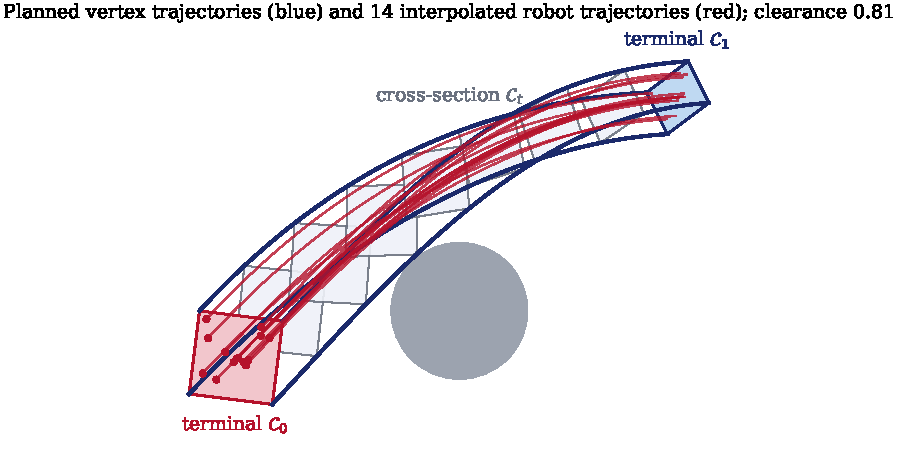
\includegraphics[width=0.9\linewidth]{virtual-tube}
  \caption{A linear virtual tube with convex-hull terminals. Only the four vertex
           trajectories (blue) are planned; each robot starts at a convex
           combination of the vertices of $\mathcal{C}_0$ and follows the same
           combination of the vertex trajectories (red).}
  \label{fig:virtual-tube}
\end{figure}

\Cref{fig:virtual-tube} shows the geometric structure of a virtual tube. The
start region (terminal $\mathcal{C}_0$) and the goal region (terminal
$\mathcal{C}_1$) are the entry and exit sets of the swarm. Each robot moves
along a trajectory $\mathbf{h}\bigl((\mathbf{q}_0, \mathbf{q}_m), t\bigr)$ from
its start point $\mathbf{q}_0$ to its exit point $\mathbf{q}_m$, and the shaded
polygons are cross-sections $\mathcal{C}_t$ of the tube at several times. Because
every cross-section is convex and the tube avoids the obstacle, any robot that
starts inside $\mathcal{C}_0$ stays inside the tube and away from the obstacle,
and many robots can pass through it at the same time.

\subsection{The Concept of Virtual Tubes}

A virtual tube is a bounded region of free space that connects the start and goal
regions and is constructed to maximize the safety margin and maintain acceptable
cross sections along the path, so that many robots can pass through
simultaneously without deadlock. Once the tube is available, path planning
reduces to assigning each robot a feasible path that stays inside the corridor
and respects minimum distances, which greatly simplifies downstream control and
coordination \cite{mao2023optimal}.

\subsubsection{Definition and Components}

Formally, a virtual tube $T$ in an $n$-dimensional configuration space is a
4-tuple $(\mathcal{C}_0, \mathcal{C}_1, f, h)$ \cite{mao2023optimal}. The
terminals $\mathcal{C}_0$ and $\mathcal{C}_1$ are disjoint, bounded, convex sets
(convexity makes them simply connected); $f : \mathcal{C}_0 \to \mathcal{C}_1$ is
a diffeomorphism that pairs every start point with an exit point, producing the
ordered pairs $\mathcal{P} = \{(\mathbf{q}_0, \mathbf{q}_m) : \mathbf{q}_0 \in
\mathcal{C}_0,\ \mathbf{q}_m = f(\mathbf{q}_0)\}$; and
$h : \mathcal{P} \times [0,1] \to T$ is a smooth map that generates the
trajectory of each pair. The cross-section at time $t$ is
$\mathcal{C}_t = \{h((\mathbf{q}_0,\mathbf{q}_m), t) : (\mathbf{q}_0,\mathbf{q}_m)
\in \mathcal{P}\}$, and every cross-section is simply connected and varies
continuously. Earlier definitions built around a generator curve are special
cases. The space is $n$-dimensional rather than three-dimensional because the
motion of a rigid robot in 3-D is described by a six-dimensional manifold.
In words:
\begin{itemize}
  \item \lead{Terminals} The start and goal regions, which delimit the entry and
        exit sets of the swarm and are chosen as simple bounded regions so that
        they can be filled without conflicts.
  \item \lead{Mapping and assignment} Establishing entry--exit pairs between the
        entry points in the start region and the exit points in the goal region,
        which are often induced by a global planner that enumerates the homotopy
        classes around the obstacles.
  \item \lead{Paths and cross sections} A family of feasible paths inside the
        corridor and their instantaneous cross sections, designed to remain
        connected and sufficiently wide to prevent congestion and maintain
        separation.
\end{itemize}

\subsubsection{Linear Tubes and the Interpolation Idea}

In practice, many deployments use linear or piecewise-linear centerlines and
polyhedral cross sections, so that the interior paths of the agents can be built
from convex combinations of, or simple interpolations between, boundary
references while preserving feasibility and spacing. A tube is \emph{linear} when
both $f$ and $h$ are linear maps; in the most useful case, the linear virtual
tube with convex-hull terminals, $\mathcal{C}_0$ and $\mathcal{C}_1$ are convex
hulls (polyhedra) of finite vertex sets and $f$ maps vertex to vertex. Under the
conditions given in \cite{mao2023optimal}, every trajectory inside such a tube
that is a convex combination of optimal vertex trajectories is itself optimal.
The planner therefore solves only a few boundary problems and obtains every other
trajectory by interpolation, which reduces the cost from
$O\bigl(k(n_t,\varepsilon)\,n_t^{2}\bigr)$--$O\bigl(k(n_t,\varepsilon)\,n_t^{3}\bigr)$
per robot to $O(n_t)$ and makes the method suitable for large swarms
\cite{mao2023optimal}.

\subsection{Optimal Virtual Tube Planning}

OVTP selects safety-margin-aware corridors and a small set of reference paths,
and it then efficiently generates the many robot paths so as to minimize
congestion and computation while guaranteeing obstacle avoidance. This approach
amortizes the heavy global search over the group and replaces independent global
planning for each robot with a lightweight synthesis inside the tube \cite{mao2023optimal}.

\subsubsection{Hierarchical Planning with MPC Tracking}

A practical architecture computes the tube(s) and the reference paths centrally
and then deploys distributed controllers (e.g., MPC) on each robot to track its
assigned path and to enforce the tube and inter-robot constraints in real time
\cite{mao2023optimal}.

MPC naturally handles receding-horizon collision avoidance and adherence to the
boundaries through inequality constraints: the position of a robot is
constrained to the interior of the tube, or to a band near its boundary for
robots on the boundary. This gives formation-like cohesion and robust tracking,
and in simulations and experiments the combination outperformed formation
control and plain predictive control in obstacle-dense environments
\cite{mao2023optimal}.

\subsubsection{Objectives: Computation, Volume, and Energy}

\begin{itemize}
  \item \lead{Computation} By reusing the same corridor and a small set of
        references, the synthesis for each agent reduces to interpolation or
        projection and local smoothing, which lowers the complexity compared with
        complete replanning for every robot.
  \item \lead{Minimum cross-sectional volume} Corridors are selected to preserve a
        sufficient cross-sectional ``capacity'' at bottlenecks; margin-aware
        backbones such as the GVD or homotopic paths preserve a safe tube
        thickness. Tube-\RRTstar{} measures this by the minimum gap volume, the
        volume of the smallest gap the path passes through \cite{mao2024tube}.
  \item \lead{Energy} Smooth curvature and non-crossing assignments reduce the
        demands for acceleration and turning and improve energy efficiency while
        maintaining throughput; choosing $f$ so that trajectories do not
        intersect serves the same purpose \cite{mao2023optimal}.
\end{itemize}

\subsubsection{Tube Networks for Complex Obstacles}

When a single corridor is insufficient, multiple tubes form a network that splits
the swarm into parallel routes around large obstacles and merges it again
downstream, thereby reducing congestion and delay. Designing consistent
assignments across the branches and avoiding internal crossings are essential for
preserving the distinction between the boundary and the interior and for
supporting safe merging behaviors; how to build such networks is still an open
question \cite{mao2023optimal}.

%-----------------------------------------------------------------------------
\section{Summary}\label{sec:ch3-summary}

This chapter reviewed and analyzed a wide range of path planning methods for
swarm robotic systems. These methods were divided into three broad
categories---deterministic, AI-based, and hybrid---each with its own distinctive
characteristics and applications. Based on this analysis, the following
conclusions can be drawn:
\begin{enumerate}
  \item \lead{Deterministic methods} Classical algorithms such as \Astar{} and
        cell decomposition perform reliably in static, known environments and
        guarantee that a path will be found. However, as discussed in
        \cref{sec:global-local}, these methods suffer from problems such as high
        computational cost and inflexibility in dynamic and complex environments.
        Sampling-based algorithms such as \RRTstar{} have partially addressed
        these challenges in high-dimensional spaces by striking a balance between
        speed and optimality.
  \item \lead{AI-based methods} This category---especially bio-inspired algorithms
        such as PSO and ACO---is highly compatible with swarm robotics owing to
        its distributed nature. The review showed that PSO, through its velocity
        and position update formula (\cref{eq:pso}), enables fast convergence in
        dynamic environments and, in most complex scenarios, succeeds in finding
        the shortest path and the minimum time simultaneously. In addition,
        reinforcement learning methods (RL and deep Q-learning) have shown great
        potential for navigation in unknown environments without a prior map.
  \item \lead{Hybrid methods} Hybrid approaches, which account for about 25\% of
        recent research, integrate the strengths of deterministic and intelligent
        methods in an attempt to overcome the limitations that each has on its
        own.
\end{enumerate}

Finally, the choice of an appropriate method depends strongly on the type of
mission (static or dynamic), on hardware limitations (processing and
communication), and on system priorities (time versus energy consumption). For
real-time applications and dynamic environments, hybrid and AI-based methods
(especially PSO and \RRTstar) are considered the superior options.
